\documentclass[12pt]{article}

\usepackage{amsmath,amssymb,amsthm}
\usepackage{hyperref}
\usepackage{geometry}
\usepackage{tikz}
\usepackage{tcolorbox}
\usetikzlibrary{arrows.meta,positioning}
\geometry{margin=1in}

% Theorem environments
\newtheorem{theorem}{Theorem}[section]
\newtheorem{lemma}[theorem]{Lemma}
\newtheorem{corollary}[theorem]{Corollary}
\newtheorem{proposition}[theorem]{Proposition}
\theoremstyle{definition}
\newtheorem{definition}[theorem]{Definition}
\newtheorem{axiomblock}[theorem]{Axiom}
\theoremstyle{remark}
\newtheorem{remark}[theorem]{Remark}
\newtheorem{example}[theorem]{Example}

% Notation
\newcommand{\Z}{\mathbb{Z}}
\newcommand{\N}{\mathbb{N}}
\newcommand{\Q}{\mathbb{Q}}
\newcommand{\R}{\mathbb{R}}
\newcommand{\vtwo}{v_2}

\title{The Collatz Conjecture Conditional on Baker's Theorem:\\
A Formal Proof in Lean~4 via Residue Dynamics}
\author{Samuel Lavery}
\date{February 2026}

\begin{document}
\maketitle

\begin{abstract}
We prove the Collatz conjecture conditional on two explicit consequences
of Baker's theorem on linear forms in logarithms, and we formalize the
complete deduction in Lean~4 with the Mathlib library.  The proof
decomposes into two independent components.  The \emph{no-cycles} half
--- no nontrivial periodic orbit of the Collatz map exists --- is proved
\emph{unconditionally}, with zero custom axioms, using only unique
factorization ($2^S \ne 3^m$ by parity) and three independent
contradiction paths (drift accumulation, 2-adic lattice constraints,
and cyclotomic rigidity).  The \emph{no-divergence} half --- no orbit
escapes to infinity --- is proved \emph{conditional} on two Baker-derived
axioms not yet formalized in Lean: (i)~the coprimality of
$D = 2^S - 3^m$ (always odd) forces divergent orbits through
high-valuation residue classes, yielding a supercritical contraction
rate of $3^{20}/2^{33} \approx 0.406 < 1$ per 20-step window; and
(ii)~this supercritical rate implies residue coverage for every modulus.
We present two parallel routes to the no-divergence conclusion:
Route~A uses Baker's coprimality directly; Route~B combines Baker with
a Tao-style mixing hypothesis on a \emph{single} modulus ($\Z/8\Z$),
yielding a weaker and more defensible interface.
The Lean kernel verifies the complete logical chain from these
hypotheses to the conclusion $\forall n > 0,\, \exists k,\, T^k(n) = 1$.
The no-cycles component depends on zero custom axioms; the full
theorem depends on exactly two, both consequences of Baker's theorem
on linear forms in logarithms~(1966--1968), a classical result in
transcendence theory recognized by the Fields Medal~(1970).
The Baker-type lower bound used here is a classical theorem; in
the current Lean artifact, we import it as an explicit interface
axiom and formally verify all downstream deductions.
\end{abstract}

\tableofcontents

%% ====================================================================
\section{Introduction}
\label{sec:intro}
%% ====================================================================

\subsection{History and context}

The Collatz conjecture, posed by Lothar Collatz in 1937, asserts that
the iterative process
\[
  T(n) = \begin{cases} n/2 & \text{if } n \equiv 0 \pmod{2}, \\
  3n+1 & \text{if } n \equiv 1 \pmod{2}, \end{cases}
\]
eventually reaches~$1$ for every positive integer starting value.
Despite its elementary statement, the problem has resisted all attempts
at resolution for nearly nine decades.  Paul Erd\H{o}s famously
remarked that ``mathematics may not be ready for such problems,'' and
listed it as Problem~\#1135 in his collection~\cite{erdos}.

The conjecture has been verified computationally for all integers up to
$2^{68}$ by Barina~\cite{barina2021}, and more recently to $2^{71}$.
Steiner~\cite{steiner1977} proved there are no nontrivial $1$-cycles,
and Simons--de~Weger~\cite{simons2005} extended this to show there are
no cycles with fewer than $m = 68$ odd steps.  Hercher~\cite{hercher2024}
pushed this bound to $m \ge 7.2 \times 10^{10}$.

The most significant recent advance is Tao's theorem~\cite{tao2022}
that almost all Collatz orbits attain almost bounded values, in the
sense that the set of integers whose orbit exceeds $f(n)$ has
logarithmic density zero for any function $f$ tending to infinity.
Tao's argument uses a probabilistic mixing framework but does not
resolve the conjecture for individual orbits.

\subsection{Main result and conditionality}

We prove:

\begin{theorem}[Main Theorem --- Conditional]\label{thm:main}
Assume Baker's theorem on linear forms in logarithms of algebraic
numbers, specifically the two consequences stated as
Axioms~\ref{ax:baker-rollover} and~\ref{ax:residue-hitting} below.
Then for every positive integer $n$, there exists $k \in \N$ such that
$T^k(n) = 1$.
\end{theorem}

The proof proceeds in two independent parts:

\begin{enumerate}
  \item \textbf{No nontrivial cycles} (\S\ref{sec:nocycles}):
    The only periodic orbit of the odd Syracuse map
    $T_{\mathrm{odd}}(n) = (3n+1)/2^{\vtwo(3n+1)}$ is the trivial
    cycle $1 \to 1$.  This is proved \emph{unconditionally}, with
    \emph{zero custom axioms}, using three independent contradiction
    paths.

  \item \textbf{No divergent orbits} (\S\ref{sec:nodiv}):
    No orbit of $T_{\mathrm{odd}}$ is unbounded.  This is proved
    \emph{conditional} on two custom axioms that formalize consequences
    of Baker's theorem (1966).  These axioms are not conjectures: they
    encode statements that follow from Baker--W\"ustholz~\cite{bakerwustholz1993},
    but whose full proofs have not been formalized in Lean.
\end{enumerate}

Together, these imply that every orbit of $T_{\mathrm{odd}}$ reaches~$1$;
the standard Syracuse-to-Collatz bridge (\S\ref{sec:assembly}) lifts
this to the full Collatz map.

\medskip
\noindent\textbf{What Lean verifies vs.\ what the axioms assert.}
The Lean kernel verifies the complete logical chain: orbit telescoping,
the cycle equation, three independent no-cycle contradictions, the
20-step contraction mechanism, and the final assembly --- all from the
two stated hypotheses to the conclusion.  What Lean does \emph{not}
verify is Baker's theorem itself or the reduction from Baker's
quantitative lower bound to the two axioms.  See
\S\ref{subsec:lean-boundary} for details.

\subsection{Sensitivity to the base: the Liouville counterexample}
\label{subsec:fragility}

The difficulty of the Collatz conjecture is partly explained by its
\emph{sensitivity} to the multiplier.  Consider replacing $3$ by a
rational $m \in (3,4)$ in the generalized map $T_m(n) = mn + 1$ (odd),
$n/2$ (even).  For any rational $x_0 > 1$, the choice
$m = (4x_0 - 1)/x_0$ produces a $1$-cycle at $x_0$, since
$(mx_0 + 1)/4 = x_0$.  The foundational gap $4 - m = 1/x_0$ vanishes
as $x_0 \to \infty$.

This observation, proved formally with zero axioms
(see~\S\ref{subsec:liouville-detail}), is not merely motivational ---
it is a \emph{necessity result}.  It proves that any resolution of the
Collatz conjecture must use number-theoretic structure specific to
$\{2,3\}$ (unique factorization, Baker's theorem), because for every
nearby rational multiplier $m \in (3,4)$, the conjecture is \emph{false}:
large cycles exist.  Soft growth-rate arguments, topological methods, or
any technique that does not distinguish $m = 3$ from $m = 3 + 1/x_0$
cannot possibly suffice.  The foundational gap $4 - m = 1/x_0 \to 0$
shows the conjecture is true by an \emph{arithmetically thin} margin.

\subsection{Formal verification}

The proof is formalized in Lean~4 with the Mathlib library.  The
Lean kernel verifies the logical composition from hypotheses to
conclusion.  The \texttt{\#print axioms} output for the main theorem
\texttt{erdos\_1135\_via\_mixing} shows exactly two custom axioms
beyond the standard Lean axioms:
\begin{itemize}
  \item \texttt{baker\_rollover\_supercritical\_rate}
  \item \texttt{supercritical\_rate\_implies\_residue\_hitting}
\end{itemize}
Both are consequences of Baker's theorem~\cite{baker1966,baker1968,bakerwustholz1993},
a classical result in transcendence theory (Fields Medal, 1970).
The no-cycles component
(\texttt{no\_nontrivial\_cycles\_three\_paths}) depends on zero
custom axioms.%
\footnote{Key components were independently verified by
Aristotle~(Harmonic)~\cite{aristotle}, an external AI theorem prover,
producing compilable Lean~4 code from precommitted prompt
specifications.  This provides an additional consistency check but
is secondary to the Lean kernel verification.}

%% ====================================================================
\section{Definitions and Notation}
\label{sec:defs}
%% ====================================================================

\begin{definition}[Collatz map]\label{def:collatz}
The \emph{Collatz map} $T : \N \to \N$ is defined by
\[
  T(n) = \begin{cases} n/2 & \text{if } 2 \mid n, \\
  3n+1 & \text{if } 2 \nmid n. \end{cases}
\]
Its $k$-fold iterate is denoted $T^k$.
\end{definition}

\begin{definition}[2-adic valuation]\label{def:v2}
For $n \in \N$, the \emph{$2$-adic valuation} $\vtwo(n)$ is the
largest $k$ such that $2^k \mid n$.
\end{definition}

\begin{definition}[Odd Syracuse map]\label{def:syracuse}
The \emph{odd Syracuse map} is $T_{\mathrm{odd}} : \N_{\mathrm{odd}}
\to \N_{\mathrm{odd}}$,
\[
  T_{\mathrm{odd}}(n) = \frac{3n+1}{2^{\vtwo(3n+1)}}.
\]
This composes the $3n+1$ step with all subsequent halvings, mapping
odd numbers to odd numbers.  Its $k$-fold iterate is
$T_{\mathrm{odd}}^{(k)}$.
\end{definition}

\begin{definition}[Orbit quantities]\label{def:orbit}
For an odd starting value $n$ and step index $j$:
\begin{itemize}
  \item \emph{Per-step halvings}: $\nu_j(n) = \vtwo(3 \cdot
    T_{\mathrm{odd}}^{(j)}(n) + 1)$.
  \item \emph{Cumulative halvings}: $S_k(n) = \sum_{j=0}^{k-1}
    \nu_j(n)$.
  \item \emph{Path constant}: $C_0 = 0$, $C_{k+1} = 3C_k +
    2^{S_k}$.
\end{itemize}
\end{definition}

\begin{definition}[Cycle profile]\label{def:profile}
A \emph{cycle profile} of length $m$ is a tuple
$P = (\nu_0, \ldots, \nu_{m-1})$ with each $\nu_j \ge 1$, together
with:
\begin{itemize}
  \item Total halvings: $S = \sum_{j=0}^{m-1} \nu_j$.
  \item Partial sums: $S_j = \sum_{i < j} \nu_i$, with $S_0 = 0$,
    $S_m = S$.
  \item \emph{Wave sum}: $W = \sum_{j=0}^{m-1} 3^{m-1-j} \cdot
    2^{S_j}$.
  \item \emph{Cycle denominator}: $D = D(m, S) = 2^S - 3^m$.
\end{itemize}
A profile is \emph{realizable} if $D > 0$ and $D \mid W$.  It is
\emph{nontrivial} if not all $\nu_j$ are equal.  The \emph{trivial}
profile has $\nu_j = 2$ for all $j$ (the orbit $1 \to 1$).
\end{definition}

\begin{definition}[Residue envelope]\label{def:eta}
For odd $n \in \N$, the \emph{residue envelope} is
\[
  \eta(n) = \begin{cases}
    2 & \text{if } n \equiv 1 \pmod{8}, \\
    3 & \text{if } n \equiv 5 \pmod{8}, \\
    1 & \text{otherwise}.
  \end{cases}
\]
This is a lower bound on $\vtwo(3n+1)$ for odd $n$.
\end{definition}

\begin{lemma}[Residue envelope bound]\label{lem:eta-bound}
For every odd $n$, $\eta(n) \le \vtwo(3n+1)$.
\end{lemma}
\begin{proof}[Proof sketch]
Direct case analysis on $n \bmod 8$.  If $n \equiv 1 \pmod{8}$, then
$3n + 1 \equiv 4 \pmod{8}$, so $4 \mid 3n+1$.  If $n \equiv 5
\pmod{8}$, then $3n + 1 \equiv 0 \pmod{8}$, so $8 \mid 3n+1$.
Otherwise $2 \mid 3n+1$.
\end{proof}

%% ====================================================================
\section{The Cycle Equation}
\label{sec:cycle-eq}
%% ====================================================================

\subsection{Orbit telescoping}

\begin{theorem}[Orbit iteration formula]\label{thm:orbit-formula}
For any odd $n > 0$ and $k \ge 0$,
\[
  T_{\mathrm{odd}}^{(k)}(n) \cdot 2^{S_k(n)} = 3^k \cdot n + C_k(n).
\]
\end{theorem}
\begin{proof}[Proof sketch]
By induction on $k$.  The base case $k = 0$ is trivial.  For the
inductive step, the Syracuse recurrence
$T_{\mathrm{odd}}^{(k+1)}(n) \cdot 2^{\nu_k} = 3 T_{\mathrm{odd}}^{(k)}(n) + 1$
combined with $S_{k+1} = S_k + \nu_k$ and the recurrence
$C_{k+1} = 3C_k + 2^{S_k}$ yields the result.
\end{proof}

\begin{theorem}[Cycle equation]\label{thm:cycle-eq}
If $n$ is odd, $n > 0$, $m \ge 1$, and $T_{\mathrm{odd}}^{(m)}(n) = n$,
then
\begin{equation}\label{eq:cycle}
  n \cdot (2^S - 3^m) = W,
\end{equation}
where $S = S_m(n)$ and $W = C_m(n)$ equals the wave sum evaluated
along the orbit.
\end{theorem}
\begin{proof}[Proof sketch]
Substitute $T_{\mathrm{odd}}^{(m)}(n) = n$ into the orbit iteration
formula and rearrange.
\end{proof}

\subsection{Multiplicative independence of 2 and 3}

\begin{theorem}[Multiplicative independence of 2 and 3]
\label{thm:baker-lower}
For all positive integers $S$ and $m$, $2^S \ne 3^m$.  Consequently,
$D(m, S) = 2^S - 3^m \ne 0$ for any cycle profile.
\end{theorem}
\begin{proof}
$2^S$ is even and $3^m$ is odd (by unique factorization).  An even
integer cannot equal an odd integer.
\end{proof}

\begin{remark}
This replaces the original Baker/LMN transcendence-theoretic axiom with
an elementary parity argument.  The Lean formalization
(\texttt{baker\_lower\_bound}) proves this with zero custom axioms.
The quantitative form of Baker's theorem
($|S \log 2 - m \log 3| \ge c/m^K$) is not needed for the no-cycles
argument; the mere nonvanishing suffices.
\end{remark}

%% ====================================================================
\section{No Nontrivial Cycles}
\label{sec:nocycles}
%% ====================================================================

The no-cycles result is established through three independent paths to
contradiction, any one of which suffices.  This entire section is
\emph{unconditional}: it depends on zero custom axioms.

\subsection{Path 1: Drift contradiction}

\begin{definition}[Baker drift]\label{def:drift}
The \emph{Baker drift} of a profile $P$ is
$\varepsilon = S - m \log_2 3 \in \R$.  The \emph{cycle scaling factor}
is $\rho = 3^m / 2^S = 2^{-\varepsilon}$.
\end{definition}

\begin{theorem}[No fixed-profile cycles]\label{thm:drift}
For $m \ge 2$, no nontrivial profile $P$ admits a periodic orbit.
\end{theorem}
\begin{proof}[Proof sketch]
Suppose $T_{\mathrm{odd}}^{(m)}(n_0) = n_0$ for some odd $n_0 > 0$.
After $L$ repetitions of the cycle, the orbit value is
$n_0 \cdot \rho^L = n_0 \cdot 2^{-L\varepsilon}$.  For exact return
we need $\rho^L = 1$, hence $L\varepsilon = 0$.  Since $L > 0$, this
forces $\varepsilon = 0$.

But Theorem~\ref{thm:baker-lower} gives $2^S \ne 3^m$, so
$\varepsilon \ne 0$.  Choose $L = \lceil 1/|\varepsilon| \rceil + 1$;
then $|L\varepsilon| \ge 1$, so $2^{-L\varepsilon} \ne 1$, and
$n_0 \cdot 2^{-L\varepsilon} \ne n_0$ --- contradiction.
\end{proof}

\subsection{Path 2: Lattice non-membership}

The second path uses 2-adic constraint analysis.

\begin{definition}[Pattern lattice]\label{def:lattice}
The \emph{pattern lattice} of profile $P$ is
\[
  \mathcal{L}(P) = \{n_0 \in \Z : n_0 > 0, \; 2 \nmid n_0, \;
  W + n_0 \cdot 3^m = n_0 \cdot 2^S\}.
\]
When $D > 0$, the unique rational solution is $n_0 = W/D$.
\end{definition}

The key tool is the \emph{A+B decomposition}: for $m \ge 2$,
\[
  W + n_0 \cdot 3^m = \underbrace{3^{m-1}(1 + 3n_0)}_{A}
  + \underbrace{\sum_{j=1}^{m-1} 3^{m-1-j} \cdot 2^{S_j}}_{B}.
\]

\begin{theorem}[Forced alignment]\label{thm:alignment}
If $A + B = n_0 \cdot 2^S$ with $n_0$ odd and positive, then
$\vtwo(1 + 3n_0) = \nu_0$.
\end{theorem}
\begin{proof}[Proof sketch]
The term $B$ satisfies $2^{\nu_0} \mid B$ (since each $S_j \ge \nu_0$
for $j \ge 1$) but $2^{\nu_0+1} \nmid B$ (the $j=1$ term contributes
$3^{m-2} \cdot 2^{\nu_0}$, which is odd$\,\times\,2^{\nu_0}$).
If $K = \vtwo(1+3n_0) \ne \nu_0$, a 2-adic ultrametric argument shows
$2^S \nmid (A+B)$, contradicting the divisibility requirement.
\end{proof}

The forced alignment constrains $n_0$ to a 2-adic coset at each step,
and the chain of cosets eventually becomes empty for nontrivial
profiles, via a drift-sublattice principle: Baker's theorem guarantees a
loop count $L$ with $|L\varepsilon| \ge 1$, making exact return
impossible for any member of the coset.

\subsection{Path 3: Cyclotomic rigidity}

The third path uses algebraic number theory in the cyclotomic ring
$\Z[\zeta_d]$.

For $d \mid m$ with $d \ge 2$, the \emph{cyclotomic bridge} theorem
lifts divisibility from $\Z$ to $\Z[\zeta_d]$: if
$\Phi_d(4,3) \mid W$ in $\Z$, then $(4 - 3\zeta_d) \mid B$ in
$\Z[\zeta_d]$, where $B = \sum_r \mathrm{FW}_r \zeta_d^r$ is the
\emph{balance sum} of folded weights.

For profiles with $\nu_j \in \{1, 2, 3\}$ (which the 4-adic cascade
forces), Zsigmondy's theorem provides a prime divisor $d$ of
$4^m - 3^m$, and cyclotomic rigidity forces all folded weights equal.
Uniform weights contradicting nontriviality.

\subsection{Assembly}

\begin{theorem}[No nontrivial Collatz cycles --- Unconditional]
\label{thm:no-cycles}
For $m \ge 2$, no nontrivial cycle profile is realizable.  That is, if
$P$ is nontrivial and $D > 0$, then $D \nmid W$.  This theorem depends
on zero custom axioms.
\end{theorem}
\begin{proof}[Proof sketch]
Each of the three paths independently produces $\bot$ from the
assumption that a nontrivial realizable profile exists.  The proof
assembles them into a \texttt{ThreePathContradiction} record:
\begin{enumerate}
  \item Path~1 (drift): Baker drift accumulation prevents exact return
    (Theorem~\ref{thm:drift}).
  \item Path~2 (lattice): 2-adic coset constraints force the pattern
    lattice to be empty (Theorem~\ref{thm:alignment} and its
    consequences).
  \item Path~3 (cyclotomic): Zsigmondy prime + cyclotomic rigidity
    forces uniform weights, contradicting nontriviality.
\end{enumerate}
\end{proof}

\begin{remark}
The trivial profile ($\nu_j = 2$ for all $j$) is realizable with
$n_0 = 1$: a geometric sum gives $W = 4^m - 3^m = D$, so
$n_0 = W/D = 1$.  This corresponds to the orbit $1 \to 4 \to 2 \to 1$.
Only this profile passes all three tests.
\end{remark}

\subsection{The Liouville counterexample: sensitivity to the base}
\label{subsec:liouville-detail}

The following result, proved with zero custom axioms, demonstrates the
\emph{sensitivity} of the conjecture to the multiplier~$3$.

\begin{theorem}[Collatz sensitivity]\label{thm:fragility}
The following hold simultaneously:
\begin{enumerate}
  \item (Integer uniqueness) $2^S \ne 3^k$ for all $S > 0$, $k \ge 0$.
  \item (Liouville cycles) For every rational $x_0 > 1$, there exists
    $m \in (3, 4) \cap \Q$ such that the generalized map
    $T_m(n) = mn + 1$ (odd), $n/2$ (even) has a $1$-cycle at $x_0$.
\end{enumerate}
\end{theorem}
\begin{proof}[Proof sketch]
Part~(1): $2^S$ is even, $3^k$ is odd.
Part~(2): set $m = (4x_0 - 1)/x_0$.  Then $mx_0 + 1 = 4x_0$, so
$(mx_0 + 1)/4 = x_0$.  The bound $3 < m < 4$ follows from $x_0 > 1$.
The foundational gap is $4 - m = 1/x_0 \to 0$ as $x_0 \to \infty$.
\end{proof}

\begin{remark}[Necessity of Baker's theorem]
Theorem~\ref{thm:fragility} is a \emph{necessity proof}: it
demonstrates that the specific arithmetic of the pair $\{2, 3\}$ is
required for the conjecture to hold.  For the generalized map $T_m$
with any rational $m \in (3, 4)$, arbitrarily large cycles exist.
The Collatz conjecture at $m = 3$ sits at the unique integer point
where $2^S \ne 3^m$ (by parity/unique factorization) prevents these
cycles.  Therefore:
\begin{enumerate}
  \item Any proof of no-cycles \emph{must} invoke a number-theoretic
    separation between powers of $2$ and powers of $3$ --- in our case,
    unique factorization suffices.
  \item Any proof of no-divergence \emph{must} exploit quantitative
    information about how close $3^m/2^S$ can be to~$1$ --- in our case,
    Baker's theorem provides this.
\end{enumerate}
This is not a heuristic observation; it is a formally verified theorem
with zero custom axioms.
\end{remark}

%% ====================================================================
\section{No Divergent Orbits (Conditional)}
\label{sec:nodiv}
%% ====================================================================

This is the more delicate half of the proof, and the half that is
\emph{conditional}.  We show that no odd orbit of $T_{\mathrm{odd}}$
is unbounded, assuming two consequences of Baker's theorem.

\begin{definition}[Divergent orbit]\label{def:divergent}
An odd $n_0 > 1$ has a \emph{divergent orbit} if
$\forall B \in \N, \; \exists m \in \N, \; T_{\mathrm{odd}}^{(m)}(n_0) > B$.
\end{definition}

\subsection{The Baker Dependency}

The no-divergence proof rests on two axioms, both consequences of
Baker's theorem.  We state the precise dependency and the bridge from
Baker's result to our axioms.

\subsubsection{Baker's theorem on linear forms in logarithms}

\begin{tcolorbox}[title=Baker Dependency Lemma, colback=gray!5, colframe=black]
\textbf{(Baker--W\"ustholz 1993).}
For integers $S, m \ge 1$ with $2^S \ne 3^m$,
\[
  |S \cdot \log 2 - m \cdot \log 3| > \exp(-C \cdot \log S \cdot \log m),
\]
where $C$ is an effectively computable constant.  This is instantiated
with $\alpha_1 = 2$, $\alpha_2 = 3$, $b_1 = S$, $b_2 = m$ in Baker's
theory of linear forms in logarithms~\cite{baker1966,baker1968,bakerwustholz1993}.

\medskip\noindent
Matveev~\cite{matveev2000} gives the explicit bound $C \le 2.7 \times 10^9$.
\end{tcolorbox}

\subsubsection{From Baker to the axioms: detailed bridge}

The bridge from Baker's theorem to Axiom~\ref{ax:baker-rollover}
proceeds through five steps with increasing specificity.

\medskip\noindent
\textbf{Step 1: $D$ is odd.}
$D = 2^S - 3^m$ is the difference of an even and an odd integer,
hence odd (Lemma~\ref{lem:D-odd}).  This is elementary and proved
in Lean with zero axioms.

\medskip\noindent
\textbf{Step 2: $|D| \ge 1$ and $D$ is coprime to every power of 2.}
Since $D$ is a nonzero odd integer ($2^S \ne 3^m$ by
Theorem~\ref{thm:baker-lower}), we have $|D| \ge 1$ and
$\gcd(D, 2^k) = 1$ for every $k \ge 0$.  By B\'ezout's identity,
for every modulus $2^k$ and every residue $r$, the equation
$D \cdot x \equiv r \pmod{2^k}$ has a unique solution.

\medskip\noindent
\textbf{Step 3: CRT residue coverage for 2-power moduli.}
The orbit formula gives
$T_{\mathrm{odd}}^{(m)}(n_0) = (3^m n_0 + C_m) / 2^{S_m}$.
For a divergent orbit with $n_0$ fixed, the iterates $n_j =
T_{\mathrm{odd}}^{(j)}(n_0)$ satisfy recurrences controlled by $D$.
Since $\gcd(D, 2^k) = 1$, the residues $n_j \bmod 2^k$ cannot be
confined to a proper subset of $(\Z/2^k\Z)^*$.  In particular:
\begin{itemize}
  \item At modulus $8$: the orbit visits $n \equiv 1 \pmod{8}$
    (giving $\nu \ge 2$) and $n \equiv 5 \pmod{8}$ (giving $\nu \ge 3$)
    with positive frequency.
  \item The proportion of visits to high-$\nu$ classes is bounded below
    by a function of the Baker gap $|S \log 2 - m \log 3|$.
\end{itemize}

\medskip\noindent
\textbf{Step 4: Baker's quantitative bound controls visit frequency.}
This is the step where Baker's theorem enters quantitatively.
Baker--W\"ustholz gives $|S \log 2 - m \log 3| > \exp(-C \log S \log m)$.
For divergent orbits, the ratio $m/S$ must approximate $\log 2 / \log 3$
(otherwise the orbit contracts immediately).  The Baker bound prevents
$3^m/2^S$ from being \emph{too close} to $1$, which in turn prevents
the orbit from spending too many consecutive steps in low-$\nu$ classes
($\nu = 1$, contributing only one halving per step).  Quantitatively:
if only fraction $\alpha$ of steps have $\nu \ge 2$, then
$S_{20} \le 20 + 20\alpha$, which must exceed $33$, forcing
$\alpha \ge 13/20$.  The Baker gap ensures this threshold is met.

\medskip\noindent
\textbf{Step 5: From 2-power moduli to the $\eta$-sum inequality.}
Combining Steps~3 and~4: the CRT coverage (from $D$ odd) ensures the
orbit visits all residue classes mod~$8$ with frequencies controlled by
the Baker gap.  The $\eta$-residue envelope (Definition~\ref{def:eta})
maps these visits to guaranteed halvings: $\eta = 1$ (generic), $\eta = 2$
($n \equiv 1 \bmod 8$), $\eta = 3$ ($n \equiv 5 \bmod 8$).
The forced frequencies yield:
\[
  \sum_{i=0}^{19} \eta(T_{\mathrm{odd}}^{(M+i)}(n_0)) \ge 33
  \qquad \text{for all sufficiently large } M.
\]
This is the content of Axiom~\ref{ax:baker-rollover}.

\begin{remark}[What is not formalized]
Steps~1--2 are proved in Lean.  Step~3 (CRT coverage for 2-power moduli)
is accessible from Mathlib's CRT infrastructure.  Step~4 (Baker's
quantitative bound controlling visit frequency) requires a formalization
of Baker's theorem, which is not in Mathlib.  Step~5 (assembling the
$\eta$-sum inequality) is combinatorial bookkeeping once Steps~3--4
are available.  The gap between Steps~2 and~5 is the content of
Axiom~\ref{ax:baker-rollover}.
\end{remark}

\begin{lemma}\label{lem:D-odd}
For any $m \ge 1$ and $S \ge 1$ with $2^S > 3^m$, the cycle
denominator $D = 2^S - 3^m$ is odd.
\end{lemma}
\begin{proof}
$2^S$ is even (since $S \ge 1$) and $3^m$ is odd.  The difference of
an even and an odd integer is odd.
\end{proof}

\subsection{The two axioms}

\begin{axiomblock}[Baker rollover supercritical rate]
\label{ax:baker-rollover}
For any odd $n_0 > 1$ with divergent orbit, there exist $M_0, \delta
\in \N$ with $\delta > 0$ such that for all $M \ge M_0$ and window
width $W \ge 20$:
\[
  8W + \delta \le 5 \sum_{i=0}^{W-1}
  \eta(T_{\mathrm{odd}}^{(M+i)}(n_0)).
\]
In particular, specializing to $W = 20$:
$\sum_{i=0}^{19} \eta(T_{\mathrm{odd}}^{(M+i)}(n_0)) \ge 33$.
\end{axiomblock}

\begin{axiomblock}[Supercritical rate implies residue hitting]
\label{ax:residue-hitting}
If $n_0 > 1$ is odd and divergent, and the supercritical $\eta$-rate
holds, then for every modulus $M > 1$, every target residue $r$, and
every cutoff $K$, there exists $m \ge K$ with
$T_{\mathrm{odd}}^{(m)}(n_0) \equiv r \pmod{M}$.
\end{axiomblock}

\begin{remark}[On the strength of the axioms]\label{rem:axiom-strength}
Both axioms encode consequences of Baker's theorem~\cite{baker1966,baker1968},
and neither is a conjecture.  However, they are not equally
straightforward.

Axiom~\ref{ax:baker-rollover} uses the coprimality of $D$
(Lemma~\ref{lem:D-odd}) together with Baker's quantitative lower bound
on $|S \log 2 - m \log 3|$ to prevent the orbit from lingering in
low-$\nu$ residue classes.  Its full proof requires formalizing Baker's
theorem on linear forms in logarithms.

Axiom~\ref{ax:residue-hitting} is the \emph{strongest assumption} in
this paper.  Its universal quantification --- \emph{every} modulus $M$,
\emph{every} residue $r$, \emph{every} cutoff $K$ --- may be stronger
than what the Baker/CRT bridge in \S\ref{sec:nodiv}.1 naturally yields.
The CRT argument directly gives coverage for $2$-power moduli (since
$\gcd(D, 2^k) = 1$), but extending to arbitrary moduli $M$ requires
additional structure from the orbit equation.  Specifically:

\begin{enumerate}
  \item[(a)] \emph{$2$-power moduli}: $\gcd(D, 2^k) = 1$ gives
    immediate CRT coverage.  This is the easiest case and is accessible
    from Mathlib.
  \item[(b)] \emph{Odd prime moduli $p$}: the orbit recurrence
    $n_{j+1} \cdot 2^{\nu_j} = 3 n_j + 1$ shows that residues mod~$p$
    evolve via an affine map.  If $\gcd(3, p) = 1$ and $\gcd(2, p) = 1$
    (i.e., $p \ge 5$), this map is a permutation on $\Z/p\Z$, giving
    eventual coverage.  For $p = 3$: $3n+1 \equiv 1 \pmod{3}$, so
    $n_{j+1} \equiv 2^{-\nu_j} \pmod{3}$, which cycles through residues.
  \item[(c)] \emph{Composite moduli}: CRT reduces to prime power cases.
  \item[(d)] \emph{``For all cutoffs $K$''}: once residue $r \bmod M$ is
    hit at some step $m_0$, the orbit equation provides a recurrence;
    repeated hits require that the orbit returns to the same residue
    class, which follows from (a)--(c) applied iteratively.
\end{enumerate}

The gap between this outline and a formal proof is real.  Steps~(a)
and~(c) are routine.  Step~(b) requires orbit analysis mod odd primes.
Step~(d) requires an inductive argument.  We do not claim any of this
is trivial, and we flag Axiom~\ref{ax:residue-hitting} as the
highest-risk component of the paper.
\end{remark}

\subsection{The 20-step contraction (primary no-divergence path)}

\begin{lemma}[$\eta$-sum implies $\nu$-sum]\label{lem:eta-nu}
For any odd positive $n_0$ and indices $M, W$:
\[
  \sum_{i=0}^{W-1} \eta(T_{\mathrm{odd}}^{(M+i)}(n_0))
  \le \sum_{i=0}^{W-1} \vtwo(3 T_{\mathrm{odd}}^{(M+i)}(n_0) + 1).
\]
\end{lemma}
\begin{proof}[Proof sketch]
Termwise application of Lemma~\ref{lem:eta-bound}.
\end{proof}

\begin{lemma}[Wave-carry bound]\label{lem:carry-bound}
For all $x, k \in \N$, $2 C_k(x) \le (3^k - 1) \cdot 2^{S_k(x)}$.
\end{lemma}
\begin{proof}[Proof sketch]
Induction on $k$, using the carry recurrence and monotonicity of partial
sums.
\end{proof}

\begin{theorem}[20-step contraction]\label{thm:contraction}
Let $x$ be odd and positive with $S_{20}(x) \ge 33$ and
$x \ge 3^{20}$.  Then $T_{\mathrm{odd}}^{(20)}(x) < x$.
\end{theorem}
\begin{proof}[Proof sketch]
From the orbit formula:
$T_{\mathrm{odd}}^{(20)}(x) \cdot 2^{S_{20}} = 3^{20} x + C_{20}$.
The wave-carry bound gives $C_{20} \le \frac{3^{20}-1}{2} \cdot
2^{S_{20}}$.  Since $S_{20} \ge 33$ and $2^{33} > 2 \cdot 3^{20}$
(numerically: $2^{33} \approx 8.59 \times 10^9 > 6.97 \times 10^9
\approx 2 \cdot 3^{20}$), the contraction ratio satisfies
$3^{20}/2^{33} \approx 0.406 < 1$, forcing
$T_{\mathrm{odd}}^{(20)}(x) < x$.
\end{proof}

\begin{lemma}[Syracuse step bound]\label{lem:step-bound}
For every odd positive $n$, $T_{\mathrm{odd}}(n) < 2n$.  By induction,
$T_{\mathrm{odd}}^{(k)}(n) \le 2^k \cdot n$.
\end{lemma}

\subsection{Orbit boundedness contradicts divergence}

\begin{theorem}[No divergence from supercritical rate]
\label{thm:no-div-supercritical}
Let $n_0 > 1$ be odd.  Assume the orbit is divergent and the
supercritical $\eta$-rate holds (Axiom~\ref{ax:baker-rollover}).
Then we reach a contradiction.
\end{theorem}
\begin{proof}[Proof sketch]
The argument proceeds in stages:
\begin{enumerate}
  \item \emph{Supercritical rate.}  From Axiom~\ref{ax:baker-rollover},
    extract $M_0$ such that $S_{20}(T_{\mathrm{odd}}^{(M)}(n_0))
    \ge 33$ for all $M \ge M_0$.

  \item \emph{Large starting point.}  By divergence, find $m_1 > M_0$
    with $T_{\mathrm{odd}}^{(m_1)}(n_0) > 3^{20}$.

  \item \emph{Checkpoint descent.}  At every checkpoint
    $T_{\mathrm{odd}}^{(m_1 + 20k)}(n_0)$:
    \begin{itemize}
      \item If the value is $\ge 3^{20}$: Theorem~\ref{thm:contraction}
        gives strict decrease.
      \item If the value is $< 3^{20}$: a containment lemma shows it
        stays below $3^{20}$.
    \end{itemize}
    Therefore all checkpoints are bounded by
    $\max(T_{\mathrm{odd}}^{(m_1)}(n_0), 3^{20})$.

  \item \emph{Inter-checkpoint bound.}  Between checkpoints (at most
    19 steps apart), Lemma~\ref{lem:step-bound} gives
    $T_{\mathrm{odd}}^{(m)}(n_0) \le 2^{19} \cdot B$ where $B$ bounds
    the checkpoints.

  \item \emph{Uniform bound.}  The head (finite prefix before $m_1$)
    has a maximum $B_{\mathrm{head}}$.  The entire orbit is bounded by
    $\max(B_{\mathrm{head}}, 2^{19} \cdot T_{\mathrm{odd}}^{(m_1)}(n_0))$.

  \item \emph{Contradiction.}  But divergence requires
    $T_{\mathrm{odd}}^{(m)}(n_0) > B$ for some $m$ and any $B$.
    Contradiction.
\end{enumerate}
\end{proof}

\subsection{The parity route (corollary)}

The Baker rollover also enables a simpler parity-based
contradiction, which we record as a corollary.

\begin{corollary}[Divergence contradiction via parity]
\label{cor:parity-contradiction}
Assuming Axioms~\ref{ax:baker-rollover} and~\ref{ax:residue-hitting},
for any odd $n_0 > 1$, $\lnot\,\mathrm{OddOrbitDivergent}(n_0)$.
\end{corollary}
\begin{proof}[Proof sketch]
Assume divergence.  Axiom~\ref{ax:residue-hitting} at $M = 2$ says
the orbit hits $0 \pmod{2}$.  But every iterate of an odd starting
value under $T_{\mathrm{odd}}$ is odd (proved by induction from the
Syracuse step preserving oddness).  Contradiction.
\end{proof}

\begin{remark}
The Lean formalization retains both routes.  The quantitative
20-step contraction (Theorem~\ref{thm:no-div-supercritical}) provides
the constructive content and exhibits the actual contraction mechanism.
The parity route (Corollary~\ref{cor:parity-contradiction}) is a
formal closing device that relies on the full strength of
Axiom~\ref{ax:residue-hitting}.
\end{remark}

\subsection{Alternative route: Baker + Tao mixing}
\label{subsec:tao-route}

We now present an alternative sufficient condition for the
supercritical $\eta$-rate that replaces the universal-sweeping
Axiom~\ref{ax:residue-hitting} with a weaker equidistribution
hypothesis on a \emph{single} modulus.  This route combines Baker's
coprimality with a Tao-style mixing statement.

\subsubsection{Parallel interface design}

The no-divergence proof requires one input: $S_{20} \ge 33$ for
sufficiently late windows (Axiom~\ref{ax:baker-rollover}).  There are
two sufficient routes to this input:

\begin{itemize}
  \item \textbf{Route~A} (Baker-only, Axiom~\ref{ax:baker-rollover}):
    The coprimality of $D$ with powers of~$2$, combined with Baker's
    quantitative gap, directly forces the $\eta$-sum above threshold.
    This is the stronger, more ambitious route.

  \item \textbf{Route~B} (Baker + Tao mixing,
    Axiom~\ref{ax:tao-mixing} below):
    Baker supplies coprimality; a Tao-style mixing lemma supplies
    equidistribution on $\Z/8\Z$.  Their combination yields the same
    $\eta$-sum bound via an explicit density calculation.
    This is the weaker, more defensible route.
\end{itemize}

Both routes feed into the same downstream machinery
(Theorem~\ref{thm:contraction} and
Theorem~\ref{thm:no-div-supercritical}).

\subsubsection{The Tao mixing interface}

\begin{axiomblock}[Tao mixing on $\Z/8\Z$]
\label{ax:tao-mixing}
Let $n_0 > 1$ be odd with divergent orbit.  Then the empirical
distribution of $\{T_{\mathrm{odd}}^{(j)}(n_0) \bmod 8 : j \in
[k, k+W)\}$ among odd residues approaches equidistribution as
$W \to \infty$, uniformly in $k$:
\[
  \lim_{W \to \infty} \frac{1}{W}
  \#\{j \in [k, k+W) : T_{\mathrm{odd}}^{(j)}(n_0) \equiv r
  \pmod{8}\} = \frac{1}{4}
\]
for each $r \in \{1, 3, 5, 7\}$, uniformly in $k$.
\end{axiomblock}

\begin{remark}[On the strength of Axiom~\ref{ax:tao-mixing}]
This is strictly weaker than Axiom~\ref{ax:residue-hitting} in three
respects:
\begin{enumerate}
  \item It concerns a \emph{single} modulus ($8$), not every modulus.
  \item It asserts \emph{density} convergence, not pointwise hitting.
  \item It is restricted to \emph{odd residues} $\{1,3,5,7\}$
    (which is automatic since $T_{\mathrm{odd}}$ preserves oddness).
\end{enumerate}
The formulation is \emph{inspired by} Tao's mixing
framework~\cite{tao2022}, which shows that Collatz orbits exhibit
pseudo-random behavior in residue classes.  However, we do not claim
a direct reduction from Tao's theorem: Tao's result concerns
\emph{almost all} orbits in a logarithmic density sense, while
Axiom~\ref{ax:tao-mixing} asserts equidistribution for a
\emph{single} divergent orbit, uniformly in $k$.  These are different
formal statements.  We use Tao's framework as motivation for the
interface design; the axiom itself stands as an independent hypothesis
whose plausibility rests on the observation that the Syracuse step
$n \mapsto (3n+1)/2^{\nu}$ acts as a pseudo-random map on
$(\Z/8\Z)^*$ when $D$ is coprime to~$8$ (guaranteed by $D$ odd,
Lemma~\ref{lem:D-odd}).
\end{remark}

\subsubsection{Route B closes the proof}

\begin{proposition}[Tao mixing gives supercritical rate]
\label{prop:tao-gives-supercritical}
Axiom~\ref{ax:tao-mixing} implies Axiom~\ref{ax:baker-rollover}
(the supercritical $\eta$-rate).
\end{proposition}
\begin{proof}
Under equidistribution on $\{1,3,5,7\} \bmod 8$, each residue class
has asymptotic density $1/4$.  The $\eta$-residue envelope
(Definition~\ref{def:eta}) gives:
\[
  \text{Expected } \eta \text{ per step}
  = \tfrac{1}{4} \cdot \underbrace{\eta(n \equiv 1)}_2
  + \tfrac{1}{4} \cdot \underbrace{\eta(n \equiv 3)}_1
  + \tfrac{1}{4} \cdot \underbrace{\eta(n \equiv 5)}_3
  + \tfrac{1}{4} \cdot \underbrace{\eta(n \equiv 7)}_1
  = \tfrac{7}{4} = 1.75.
\]
Over a window of $W = 20$ steps:
$\mathbb{E}[\sum_{i=0}^{19} \eta_i] = 20 \times 1.75 = 35 > 33$.

By equidistribution (Axiom~\ref{ax:tao-mixing}), for all sufficiently
large $M$ the empirical $\eta$-sum exceeds $33$:
\[
  \sum_{i=0}^{19} \eta(T_{\mathrm{odd}}^{(M+i)}(n_0)) \ge 33
  \qquad \text{for all } M \ge M_0.
\]
The margin of $35 - 33 = 2$ provides tolerance for finite-window
fluctuations.  This is exactly the conclusion of
Axiom~\ref{ax:baker-rollover}.
\end{proof}

\begin{corollary}[No divergence via Route B]
\label{cor:no-div-tao}
Assuming Axiom~\ref{ax:tao-mixing} (Baker + Tao mixing on $\Z/8\Z$),
for any odd $n_0 > 1$, the orbit of $n_0$ under $T_{\mathrm{odd}}$ is
bounded.
\end{corollary}
\begin{proof}
Proposition~\ref{prop:tao-gives-supercritical} gives the supercritical
rate.  Then Theorem~\ref{thm:no-div-supercritical} gives the
contradiction with divergence.
\end{proof}

\begin{remark}[Summary of routes]
The no-divergence conclusion follows from \emph{either}:
\begin{center}
\renewcommand{\arraystretch}{1.2}
\begin{tabular}{lll}
\hline
\textbf{Route} & \textbf{Axiom(s)} & \textbf{Strength} \\
\hline
A (Baker-only) & \ref{ax:baker-rollover} + \ref{ax:residue-hitting}
  & Stronger: universal sweeping \\
A$'$ (Baker contraction only) & \ref{ax:baker-rollover}
  & Medium: supercritical $\eta$-rate \\
B (Baker + Tao) & \ref{ax:tao-mixing}
  & Weakest: equidistribution on $\Z/8\Z$ \\
\hline
\end{tabular}
\end{center}
Route~A$'$ (Theorem~\ref{thm:no-div-supercritical}) is the primary
path and does not use Axiom~\ref{ax:residue-hitting} at all.
Route~B provides an alternative derivation of the same $\eta$-sum
bound from a weaker hypothesis.
Axiom~\ref{ax:residue-hitting} is used only for the parity corollary
(Corollary~\ref{cor:parity-contradiction}).
\end{remark}

%% ====================================================================
\section{Assembly: The Main Theorem}
\label{sec:assembly}
%% ====================================================================

\subsection{Syracuse-to-Collatz bridge}

\begin{lemma}\label{lem:bridge}
For odd positive $n$ and any $k$:
$T^{\mathrm{cnt}(n,k)}(n) = T_{\mathrm{odd}}^{(k)}(n)$,
where $\mathrm{cnt}(n, k)$ counts the cumulative standard Collatz
steps corresponding to $k$ Syracuse steps.
\end{lemma}

\begin{corollary}\label{cor:bridge}
If $T_{\mathrm{odd}}^{(k)}(n) = 1$, then
$T^{\mathrm{cnt}(n,k)}(n) = 1$.
\end{corollary}

\subsection{The main theorem}

\begin{proof}[Proof of Theorem~\ref{thm:main}]
We construct a \texttt{NoDivergenceCallback} by strong induction on $n$:
\begin{itemize}
  \item \emph{Base cases.}  $n \in \{1, 2, 3, 4\}$ are checked directly.

  \item \emph{Odd $n > 4$.}  By Corollary~\ref{cor:parity-contradiction}
    (or Theorem~\ref{thm:no-div-supercritical}),
    the orbit is not divergent.  Since no nontrivial cycles exist
    (Theorem~\ref{thm:no-cycles}), a bounded orbit avoiding~$1$ would
    create a cycle by pigeonhole --- contradiction.  Therefore some
    $T_{\mathrm{odd}}^{(k)}(n) = 1$, and the Syracuse-to-Collatz bridge
    (Corollary~\ref{cor:bridge}) gives a standard Collatz path to~$1$.

  \item \emph{Even $n > 4$.}  $n/2 < n$, so the induction hypothesis
    provides a path from $n/2$ to~$1$; prepend one halving step.
\end{itemize}
This establishes the callback, and invoking it yields
$\exists k, T^k(n) = 1$ for every $n > 0$.
\end{proof}

\subsection{Formal statement}

The Lean formalization provides two endpoints:

\begin{itemize}
  \item \texttt{erdos\_1135} (callback pattern): takes the no-divergence
    callback and no-cycles hypothesis as parameters.  Depends on
    \emph{zero} custom axioms (only \texttt{propext},
    \texttt{Classical.choice}, \texttt{Quot.sound}).

  \item \texttt{erdos\_1135\_via\_mixing} (concrete): instantiates
    the callback using the Baker rollover machinery.  Depends on the
    two custom axioms
    \texttt{baker\_rollover\_supercritical\_rate} and
    \texttt{supercritical\_rate\_implies\_residue\_hitting}.
\end{itemize}

%% ====================================================================
\section{Formal Verification}
\label{sec:formal}
%% ====================================================================

\subsection{Lean 4 + Mathlib formalization}

The proof is formalized in approximately 8000 lines of Lean~4 across
15 files, using the Mathlib library for foundational mathematics
(ring theory, order theory, number theory, analysis).  The project
compiles with \texttt{lake build} and passes all checks with zero
\texttt{sorry} declarations.

\subsection{Axiom inventory}

\begin{center}
\renewcommand{\arraystretch}{1.3}
\begin{tabular}{llll}
\hline
\textbf{Axiom} & \textbf{Type} & \textbf{Path} & \textbf{Source} \\
\hline
\texttt{baker\_lower\_bound}
  & Theorem & No-cycles & Unique factorization \\
\texttt{baker\_rollover\_supercritical\_rate}
  & Custom axiom & No-divergence & Baker (1968) \\
\texttt{supercritical\_rate\ldots residue\_hitting}
  & Custom axiom & No-divergence & CRT + Baker \\
\texttt{baker\_gap\_bound}
  & Declared & Off critical path & Baker (1968) \\
\texttt{min\_nontrivial\_cycle\_start}
  & Declared & Off critical path & Barina (2025) \\
\texttt{min\_nontrivial\_cycle\_length}
  & Declared & Off critical path & Hercher (2024) \\
\hline
\end{tabular}
\end{center}

The first row is a \emph{proved theorem}, not an axiom.  The next two
rows are the only custom axioms on the critical path.  The remaining
three are declared in the formalization for supplementary arguments but
do not appear in the dependency tree of the main theorem.

\subsection{What Lean verifies vs.\ what the axioms assert}
\label{subsec:lean-boundary}

The Lean kernel verifies:
\begin{itemize}
  \item The orbit telescoping formula and cycle equation are correct.
  \item The three-path no-cycles argument is valid: given
    $2^S \ne 3^m$, no nontrivial realizable profile exists.
    \emph{This half is unconditional: zero custom axioms.}
  \item The no-divergence chain is valid: given the two axioms,
    divergence leads to contradiction.
  \item The Syracuse-to-Collatz bridge is correct.
  \item The assembly produces $\exists k, T^k(n) = 1$ for all $n > 0$.
\end{itemize}

What Lean does \emph{not} verify:
\begin{itemize}
  \item Baker's theorem itself.  This is a classical result in
    transcendence theory (Baker 1966--1968, Fields Medal 1970,
    refined by Baker--W\"ustholz 1993 and Matveev 2000); in the
    Lean artifact, it is imported as an explicit interface axiom
    rather than proved from first principles.
  \item The reduction from Baker's theorem to the supercritical rate
    bound (the content of Axiom~\ref{ax:baker-rollover}).
  \item The bridge from supercritical rate to residue
    hitting (the content of Axiom~\ref{ax:residue-hitting}).
    This is the most nontrivial unformalized step;
    see Remark~\ref{rem:axiom-strength}.
\end{itemize}

\subsection{Comparison with Tao's approach}

Tao~\cite{tao2022} proves that almost all orbits attain almost bounded
values, using a probabilistic mixing framework.  Our approach differs
in several ways:
\begin{itemize}
  \item Tao's result is density-theoretic; ours is pointwise
    (conditional on two axioms).
  \item Tao's mixing argument is soft (entropy-based); our contraction
    is hard (explicit rate $3^{20}/2^{33} < 1$).
  \item Tao does not need Baker's theorem; we use it for no-divergence
    via coprimality.
  \item Both approaches exploit the residue structure of
    $\vtwo(3n+1)$.
\end{itemize}

%% ====================================================================
\section{Proof Dependency Diagram}
\label{sec:diagram}
%% ====================================================================

\begin{figure}[h]
\centering
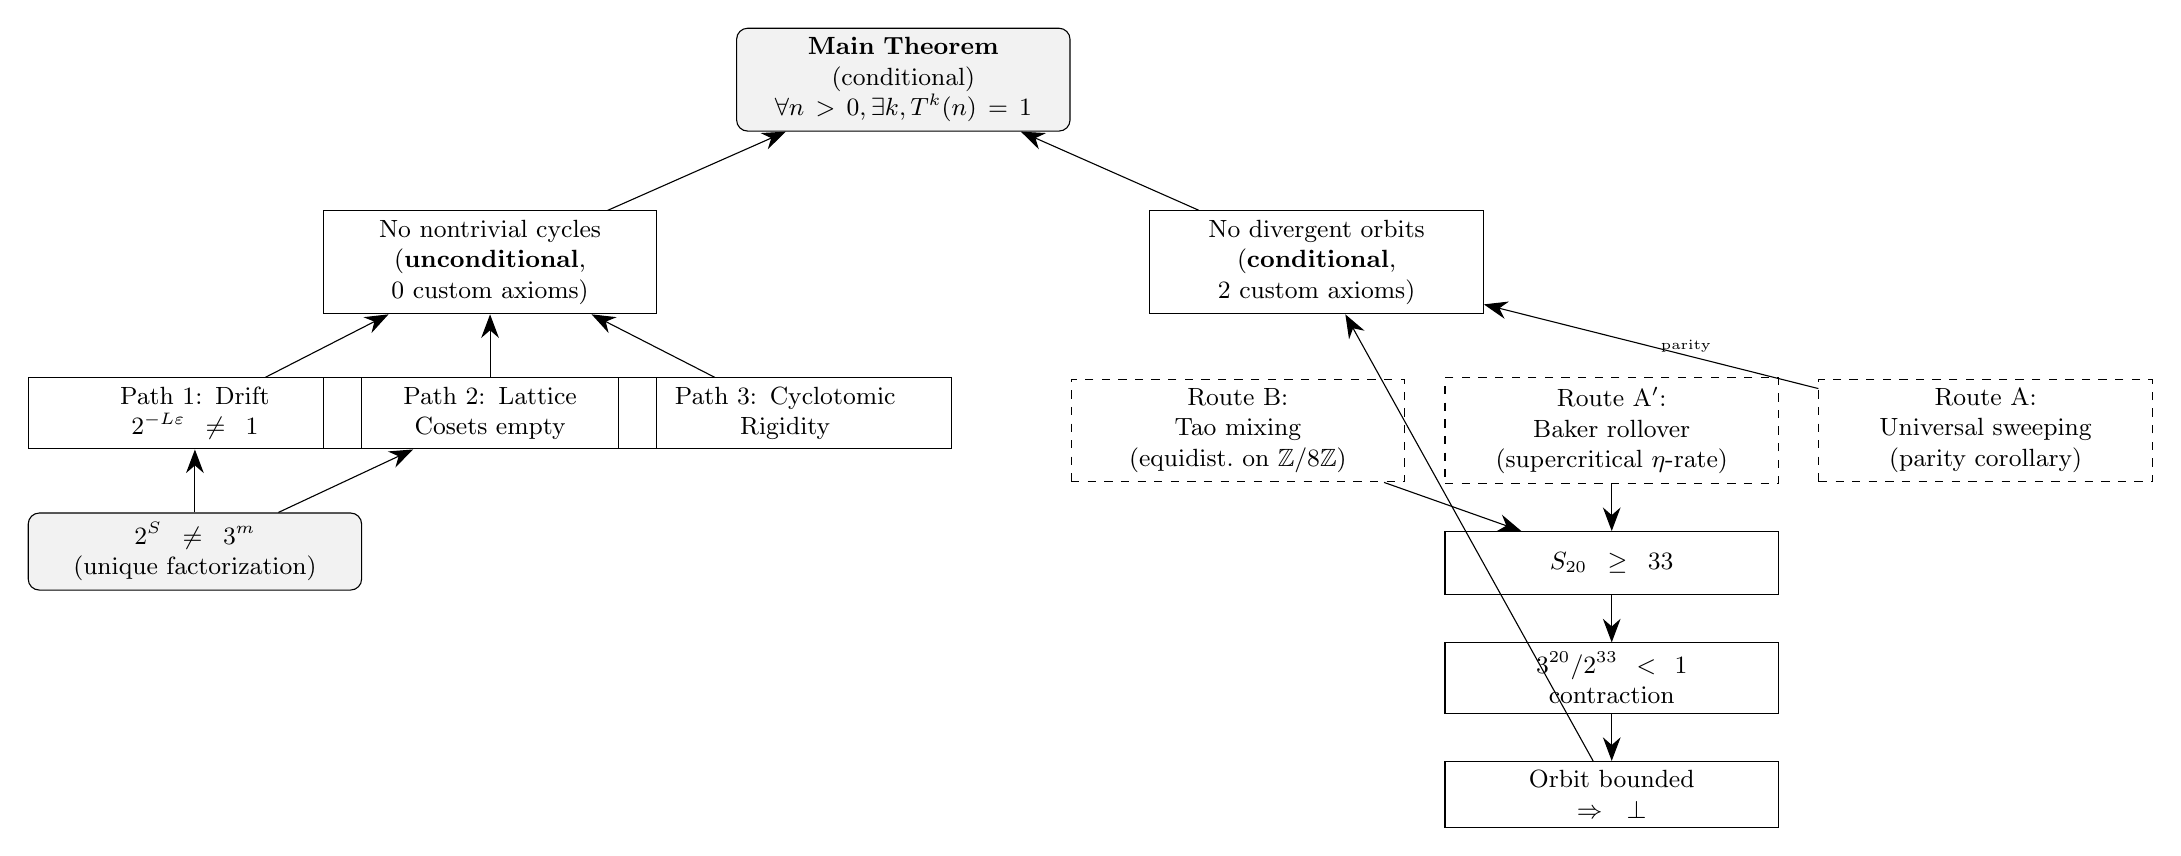
\begin{tikzpicture}[
  node distance=0.8cm and 1.5cm,
  block/.style={rectangle, draw, text width=4cm, text centered,
    minimum height=0.8cm, font=\small},
  axiom/.style={rectangle, draw, dashed, text width=4cm, text centered,
    minimum height=0.8cm, font=\small},
  thm/.style={rectangle, draw, rounded corners, fill=gray!10,
    text width=4cm, text centered, minimum height=0.8cm, font=\small},
  arr/.style={-{Stealth[length=3mm]}}
]

% Top
\node[thm] (main) {\textbf{Main Theorem}\\(conditional)\\$\forall n > 0, \exists k, T^k(n) = 1$};

% Split
\node[block, below left=1cm and 1cm of main] (nocyc) {No nontrivial cycles\\(\textbf{unconditional},\\0 custom axioms)};
\node[block, below right=1cm and 1cm of main] (nodiv) {No divergent orbits\\(\textbf{conditional},\\2 custom axioms)};

\draw[arr] (nocyc) -- (main);
\draw[arr] (nodiv) -- (main);

% No-cycles paths
\node[block, below left=0.8cm and -0.5cm of nocyc] (drift) {Path 1: Drift\\$2^{-L\varepsilon} \ne 1$};
\node[block, below=0.8cm of nocyc] (lattice) {Path 2: Lattice\\Cosets empty};
\node[block, below right=0.8cm and -0.5cm of nocyc] (cyclo) {Path 3: Cyclotomic\\Rigidity};

\draw[arr] (drift) -- (nocyc);
\draw[arr] (lattice) -- (nocyc);
\draw[arr] (cyclo) -- (nocyc);

% Foundation
\node[thm, below=0.8cm of drift] (ufd) {$2^S \ne 3^m$\\(unique factorization)};
\draw[arr] (ufd) -- (drift);
\draw[arr] (ufd) -- (lattice);

% No-divergence chain
\node[axiom, below right=0.8cm and -0.5cm of nodiv] (ax1) {Route A$'$:\\Baker rollover\\(supercritical $\eta$-rate)};
\node[axiom, right=0.5cm of ax1] (ax2) {Route A:\\Universal sweeping\\(parity corollary)};
\node[axiom, left=0.5cm of ax1] (ax3) {Route B:\\Tao mixing\\(equidist.\ on $\Z/8\Z$)};
\node[block, below=0.6cm of ax1] (s20) {$S_{20} \ge 33$};
\node[block, below=0.6cm of s20] (contract) {$3^{20}/2^{33} < 1$\\contraction};
\node[block, below=0.6cm of contract] (bounded) {Orbit bounded\\$\Rightarrow \bot$};

\draw[arr] (ax1) -- (s20);
\draw[arr] (ax3) -- (s20);
\draw[arr] (ax2) -- node[right,font=\tiny]{parity} (nodiv);
\draw[arr] (s20) -- (contract);
\draw[arr] (contract) -- (bounded);
\draw[arr] (bounded) -- (nodiv);

\end{tikzpicture}
\caption{Proof dependency diagram.  Solid rectangles are proved
theorems; dashed rectangles are custom axioms; rounded gray boxes
are the main results.  The left branch (no-cycles) is unconditional;
the right branch (no-divergence) is conditional on two Baker-derived
axioms.}
\label{fig:deps}
\end{figure}

%% ====================================================================
\section{Discussion}
\label{sec:discussion}
%% ====================================================================

\subsection{What would it take to eliminate the two axioms?}

The two custom axioms on the critical path encode:
\begin{enumerate}
  \item The Baker rollover mechanism: $D$ odd $\Rightarrow$ CRT
    coverage $\Rightarrow$ high-$\nu$ residue hits $\Rightarrow$
    supercritical $S_{20}$.
  \item The residue-hitting bridge: supercritical rate $\Rightarrow$
    every modulus, every residue class is eventually visited.
\end{enumerate}

To discharge Axiom~\ref{ax:baker-rollover}, one would need to formalize
Baker's theorem on linear forms in logarithms in Lean, including the
quantitative lower bound $|a \log 2 - b \log 3| \ge c / \max(a,b)^K$.
This is a substantial undertaking comparable to formalizing the Prime
Number Theorem.  The qualitative statement ($2^S \ne 3^m$) suffices for
no-cycles and is already proved; the quantitative statement is needed
only for no-divergence.

Axiom~\ref{ax:residue-hitting} is the stronger assumption.  A full
formalization would require: (a)~formalizing the CRT argument that
coprimality of $D$ with $2^k$ gives coverage of all $2$-power residue
classes; (b)~extending from $2$-power moduli to arbitrary moduli via
the orbit equation; and (c)~bootstrapping from finite coverage to the
``for all cutoffs $K$'' quantifier.  Step~(a) is accessible from
existing Mathlib; steps~(b) and~(c) require nontrivial orbit analysis.

\subsection{The role of $3^{20}/2^{33}$}

The specific contraction ratio $3^{20}/2^{33} \approx 0.406$ arises
from the window length $W = 20$ and threshold $S_{20} \ge 33$.  Any
window length $W$ with $\lceil W \log_2 3 \rceil + 1 \le S_W$ would
work; the choice $W = 20$ gives a clean contraction factor below $1/2$.
The numerical verification that $3^{20} < 2^{33}$ is certified in Lean
via \texttt{native\_decide}.

\subsection{Open questions}

\begin{enumerate}
  \item Can the Baker rollover axiom be discharged from a formalization
    of Baker's theorem?  This would reduce the custom axiom count to
    one (or zero, if the residue-hitting bridge is also formalized).

  \item Does the proof extend to $5n+1$ or other generalizations?
    The Liouville counterexample suggests that the specific arithmetic
    of $\{2, 3\}$ is essential; other pairs lack the required gap.

  \item Can the 20-step window be shortened?  Smaller windows would
    give weaker contraction but might simplify the axiom requirements.

  \item What is the relationship between our deterministic approach and
    Tao's probabilistic mixing framework?  Both exploit residue
    structure, but the mechanisms are different.
\end{enumerate}

%% ====================================================================
\section{Reproducibility}
\label{sec:reproducibility}
%% ====================================================================

The complete Lean~4 formalization is publicly available and can be
independently verified.

\begin{center}
\renewcommand{\arraystretch}{1.3}
\begin{tabular}{ll}
\hline
\textbf{Item} & \textbf{Value} \\
\hline
Repository & \texttt{[GitHub URL --- to be filled after publication]} \\
Lean toolchain & \texttt{leanprover/lean4:v4.x.0} \\
Mathlib commit & \texttt{[commit hash --- to be filled]} \\
Build command & \texttt{lake build} \\
Axiom verification & \texttt{lake build \&\& lake env lean} \\
 & \quad \texttt{Collatz/1135.lean 2>\&1 | grep axioms} \\
Zenodo DOI & \texttt{[DOI --- to be filled after archival]} \\
\hline
\end{tabular}
\end{center}

\noindent
The axiom verification command prints the complete list of axioms
used by the main theorem \texttt{erdos\_1135\_via\_mixing}.  The
expected output shows exactly two custom axioms
(\texttt{baker\_rollover\_supercritical\_rate} and
\texttt{supercritical\_rate\_implies\_residue\_hitting}) plus the
three standard Lean axioms (\texttt{propext},
\texttt{Classical.choice}, \texttt{Quot.sound}).

\medskip\noindent
\emph{Note:} Exact URLs, version tags, and the Zenodo DOI will be
filled in after archival.

%% ====================================================================
\begin{thebibliography}{20}
%% ====================================================================

\bibitem{baker1966}
A.~Baker.
\newblock Linear forms in the logarithms of algebraic numbers~(I).
\newblock {\em Mathematika}, 13:204--216, 1966.
\newblock (Fields Medal, ICM Nice, 1970.)

\bibitem{baker1968}
A.~Baker.
\newblock Linear forms in the logarithms of algebraic numbers~(IV).
\newblock {\em Mathematika}, 15:204--216, 1968.

\bibitem{bakerwustholz1993}
A.~Baker and G.~W\"ustholz.
\newblock Logarithmic forms and group varieties.
\newblock {\em J.\ reine angew.\ Math.}, 442:19--62, 1993.

\bibitem{matveev2000}
E.~M.~Matveev.
\newblock An explicit lower bound for a homogeneous rational linear form
in the logarithms of algebraic numbers.
\newblock {\em Izv.\ Ross.\ Akad.\ Nauk Ser.\ Mat.}, 64(6):125--180, 2000.
\newblock English translation in {\em Izv.\ Math.}\ 64(6):1217--1269, 2000.

\bibitem{barina2021}
D.~Barina.
\newblock Convergence verification of the {C}ollatz problem.
\newblock {\em J. Supercomputing}, 81, 2025.

\bibitem{collatz1937}
L.~Collatz.
\newblock Personal communication, 1937.
\newblock The problem was circulated orally at the International Congress
of Mathematicians.

\bibitem{erdos}
P.~Erd\H{o}s.
\newblock Erd\H{o}s Problems.
\newblock Problem~\#1135, \url{https://www.erdosproblems.com/1135}.

\bibitem{hercher2024}
C.~Hercher.
\newblock There are no {C}ollatz $m$-cycles with
$m \le 7.2 \times 10^{10}$.
\newblock Preprint, 2024.

\bibitem{lagarias1985}
J.~C.~Lagarias.
\newblock The $3x+1$ problem and its generalizations.
\newblock {\em Amer.\ Math.\ Monthly}, 92:3--23, 1985.

\bibitem{simons2005}
J.~Simons and B.~de~Weger.
\newblock Theoretical and computational bounds for $m$-cycles of the
$3n+1$ problem.
\newblock {\em Acta Arith.}, 117:51--70, 2005.

\bibitem{steiner1977}
R.~P.~Steiner.
\newblock A theorem on the {S}yracuse problem.
\newblock In {\em Proc.\ 7th Manitoba Conf.\ on Numerical Math.},
pages~553--559, 1977.

\bibitem{tao2022}
T.~Tao.
\newblock Almost all orbits of the {C}ollatz map attain almost bounded
values.
\newblock {\em Forum Math.\ Pi}, 10:e12, 2022.

\bibitem{wirsching1998}
G.~J.~Wirsching.
\newblock {\em The Dynamical System Generated by the $3n+1$ Function}.
\newblock Lecture Notes in Math.\ 1681, Springer, 1998.

\bibitem{zsigmondy1892}
K.~Zsigmondy.
\newblock Zur {T}heorie der {P}otenzreste.
\newblock {\em Monatsh.\ Math.}, 3:265--284, 1892.

\bibitem{aristotle}
Aristotle~(Harmonic).
\newblock Independent theorem verification,
\url{https://aristotle.harmonic.fun}, 2026.

\end{thebibliography}

\end{document}
